%% LaTeX Beamer presentation template (requires beamer package)
%% see http://bitbucket.org/rivanvx/beamer/wiki/Home
%% idea contributed by H. Turgut Uyar
%% template based on a template by Till Tantau
%% this template is still evolving - it might differ in future releases!

\documentclass{beamer}

\mode<presentation>
{
\usetheme{Warsaw}

\setbeamercovered{transparent}
}

\usepackage[english]{babel}
\usepackage[latin1]{inputenc}

% font definitions, try \usepackage{ae} instead of the following
% three lines if you don't like this look
\usepackage{mathptmx}
\usepackage[scaled=.90]{helvet}
\usepackage{courier}

\usepackage[T1]{fontenc}

% User packages
\usepackage[absolute,overlay]{textpos}
\usepackage{tikz}
\usepackage{listings}

\title{Birdhouse - supporting Web Processing Services}

%\subtitle{}

% - Use the \inst{?} command only if the authors have different
%   affiliation.
\author{\vspace{2.3cm}\\
Carsten Ehbrecht\inst{1}
\and Stephan Kindermann\inst{1}
\and Nils Hempelmann\inst{2}
}
%\author{\inst{1}}

% - Use the \inst command only if there are several affiliations.
% - Keep it simple, no one is interested in your street address.
\institute[Institute]
{
\inst{1}%
DKRZ - German Climate Compute Center
\and
\inst{2}%
GIZ - German Development Cooperation
}

\date{\footnotesize{$28^{th}$ of November 2017/ Python Frameworks Workshop at ECMWF}}


% This is only inserted into the PDF information catalog. Can be left
% out.
\subject{Talks}



% If you have a file called "university-logo-filename.xxx", where xxx
% is a graphic format that can be processed by latex or pdflatex,
% resp., then you can add a logo as follows:

% \pgfdeclareimage[height=0.5cm]{university-logo}{university-logo-filename}
% \logo{\pgfuseimage{university-logo}}



% Delete this, if you do not want the table of contents to pop up at
% the beginning of each subsection:
\AtBeginSubsection[]
{
\begin{frame}<beamer>
\frametitle{Outline}
\tableofcontents[currentsection,currentsubsection]
\end{frame}
}

% Section title slides
\AtBeginSection[]{
  \begin{frame}
  \vfill
  \centering
  \begin{beamercolorbox}[sep=8pt,center,shadow=true,rounded=true]{title}
    \usebeamerfont{title}\insertsectionhead\par%
  \end{beamercolorbox}
  \vfill
  \end{frame}
}


% If you wish to uncover everything in a step-wise fashion, uncomment
% the following command:

%\beamerdefaultoverlayspecification{<+->}

\begin{document}

\begin{frame}
   % \tikz [remember picture,overlay]
   %  \node at
   %      ([yshift=4.8cm]current page.south)
   %      %or: (current page.center)
   %      {
\includegraphics[height=2.8cm]{figures/pywps}};
   \titlepage
\end{frame}

\begin{frame}
\frametitle{Outline}
\tableofcontents
% You might wish to add the option [pausesections]
\end{frame}

% %%%%%%%%%%%%%%%%%%%%%%%%%%%%%%%%%%%%%%%%%%%%%%%%%%%%%%%%%%%%%%%%%%%%%%%%%%%%%
\section{Motivation}

%\subsection[Short First Subsection Name]{First Subsection Name}

% -----------------------------------------------
\begin{frame}
\frametitle<presentation>{The OGC Web Processing Service}

\begin{itemize}
\item OGC open web standard for remote geo-spatial processing.
\item Integrated with web data services: \textbf{WFS}, \textbf{WCS}.
\item Three basic requests:
\begin{itemize}
      \item  \textit{GetCapabilities}
      \item  \textit{DescribeProcess}
      \item  \textit{Execute}
\end{itemize}
\item Three basic input/output classes:
\begin{itemize}
      \item  \textit{Literal}
      \item  \textit{Complex} - for geo-spatial data and services
      \item  \textit{BoundingBox} - for geo-spatial data extent
\end{itemize}
\end{itemize}
\end{frame}

% -----------------------------------------------
\begin{frame}
\frametitle<presentation>{The OGC Web Processing Service}

  \begin{figure}[ht]
   \centering
   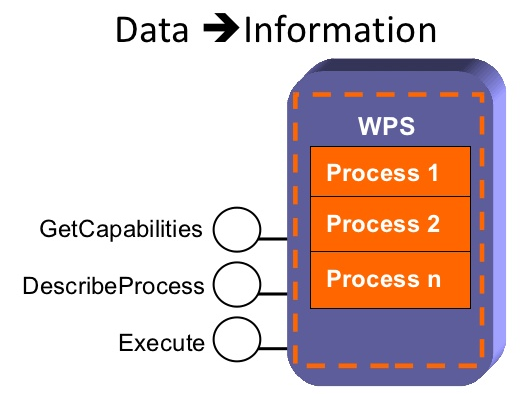
\includegraphics[height=5.85cm]{figures/WPS}
  \end{figure}

\centering
\footnotesize{http://www.slideshare.net/TheodorFoerster/restful-web-processing-service}

\end{frame}

% -----------------------------------------------
\begin{frame}
\frametitle{WPS Use Case}

  \begin{figure}[ht]
    \centering
    \includegraphics[width=11.5cm]{figures/wps_adamsteer}
  \end{figure}

\centering
\footnotesize{WPS for Point Clouds by Adam Steer, NCI, Australia}

\end{frame}

% -----------------------------------------------
\begin{frame}
\frametitle{WPS Use Case II}

  \begin{figure}[ht]
    \centering
    \includegraphics[width=11.5cm]{figures/wps-ensemble-robustness}
  \end{figure}

\end{frame}


% %%%%%%%%%%%%%%%%%%%%%%%%%%%%%%%%%%%%%%%%%%%%%%%%%%%%%%%%%%%%%%%%%%%%%%%%%%%%%
\section{PyWPS}

% -----------------------------------------------
\begin{frame}
\frametitle{What is PyWPS?}

\begin{itemize}
  \item An implementation of the OGC Web Processing Service standard
  \item Coded on the Python language (researcher friendly)
  \item Started in the Spring of 2006
  \item Supports all available tools in Python for geo-spatial operations
  \item http://pywps.org

\end{itemize}
\end{frame}


% -----------------------------------------------
\begin{frame}
\frametitle{PyWPS Scheduler Extension}

  \begin{figure}[ht]
    \centering
    \includegraphics[width=11.5cm]{figures/pywps-scheduler-extension}
  \end{figure}

  \centering
  \footnotesize{This extension is used by the CP4CDS Copernicus project}

\end{frame}


% %%%%%%%%%%%%%%%%%%%%%%%%%%%%%%%%%%%%%%%%%%%%%%%%%%%%%%%%%%%%%%%%%%%%%%%%%%%%%
\section{Birdhouse}

% -----------------------------------------------
\begin{frame}
\frametitle{What is Birdhouse?}

\begin{itemize}
  \item Supporting OGC Web Processing Services in the climate science community.
  \item http://bird-house.github.io/

\end{itemize}
\end{frame}


% -----------------------------------------------
\begin{frame}
\frametitle{Birdhouse Overview}

  \begin{figure}[ht]
    \centering
    \includegraphics[height=5.85cm]{figures/birdhouse-overview}
  \end{figure}

\end{frame}

% -----------------------------------------------
\begin{frame}
\frametitle{WSGI Application}

  \begin{figure}[ht]
    \centering
    \includegraphics[height=5.85cm]{figures/wsgi-app}
  \end{figure}

\end{frame}


% -----------------------------------------------
\begin{frame}
\frametitle{Twitcher Security Proxy}

  \begin{figure}[ht]
    \centering
    \includegraphics[height=5.85cm]{figures/twitcher}
  \end{figure}

\end{frame}


% %%%%%%%%%%%%%%%%%%%%%%%%%%%%%%%%%%%%%%%%%%%%%%%%%%%%%%%%%%%%%%%%%%%%%%%%%%%%%
\section{Summary}

\begin{frame}
\frametitle<presentation>{Summary}

\begin{itemize}

  \item Deployment
  \begin{itemize}
    \item Nginx + Gunicorn provide the infrastructure for scalable services
    \item Scalability implies increased complexity
  \end{itemize}

  \item{Docker containers}
  \begin{itemize}
    \item dockerfiles create pre-configured PyWPS images
    \item set up and deployment complexity already in place
  \end{itemize}
\end{itemize}

\end{frame}

% --------------------------------------------------------------
\begin{frame}
%\frametitle<presentation>{}

  \begin{figure}[ht]
   \centering
   
\includegraphics[height=3cm]{figures/pywps}
  \end{figure}

\centering
\Huge{Thank you!}

\vspace{0.4cm}
\normalsize{http://bird-house.github.io/}
\end{frame}

\end{document}
